\documentclass[conference]{IEEEtran}
\usepackage{cite}
\usepackage{CJKutf8}
\usepackage{amsmath,amssymb,amsfonts}
\usepackage{graphicx}
\usepackage{booktabs}
\usepackage{tabularx}
\usepackage{algorithm}
\usepackage{algpseudocode}
\usepackage{xcolor}
\usepackage{url}
\usepackage{tikz}
\usetikzlibrary{arrows.meta,positioning}
\newcolumntype{L}{>{\raggedright\arraybackslash}X}

\begin{document}
\title{Context-Aware Restaurant Recommendation with\\Taichung Bus Accessibility}

\author{
\IEEEauthorblockN{\begin{CJK}{UTF8}{bkai}林晉德、顧晏哲、魏郁倢、葉純宇\end{CJK}}
\IEEEauthorblockA{\textit{Department of Computer Science and Engineering} \\
\textit{National Chung Hsing University}\\
Taichung, Taiwan}
}
\maketitle

\begin{abstract}
A restaurant whose reviews match a user's dining occasion may still be impractical to reach because of long walks, waiting times, or transfers. Attaching a route only after a restaurant has been chosen prevents transit conditions from influencing that choice. This paper proposes a context-aware restaurant recommendation agent that considers bus accessibility in Taichung before the final ranking. A language model structures the user request, and keyword, vector, or hybrid retrieval recalls restaurants with supporting review evidence. For each candidate, bus plans are obtained from the Transport Data eXchange (TDX) service, and a program builds an arrival and dining timeline. Budget, opening-hour, walking, boarding, and transfer constraints are checked with three-valued verdicts: pass, fail, or unknown. Verified restaurant--route pairs are ranked by contextual relevance and transit burden, and explanations are generated from decision records. We also define an experimental plan covering retrieval quality, the effect of transit-aware ranking, constraint verification, and timeline modeling. This work is at the proposal stage; the expected outcome is a prototype that explains both contextual evidence and transit trade-offs.
\end{abstract}
\begin{IEEEkeywords}
restaurant recommendation, review semantics, context-aware recommendation, public bus transit, vector retrieval, knowledge graph, three-valued verification
\end{IEEEkeywords}

%=====================================================
\section{Introduction}\label{sec:intro}
Dining out is a frequent decision in daily life. By the end of 2024, Taichung City had 22,612 profit-seeking food and beverage businesses, 47.55\% more than in 2015~\cite{taichung_eat_outside}. When planning a date, a birthday celebration, or a gathering with friends, users need to know which of these restaurants suit the occasion. Reviews often contain contextual descriptions, such as ``good for conversation'' or ``romantic,'' whose wording may differ from that of the user request. Research on subjective attributes and conversational recommendation indicates the value of natural-language preferences and review evidence~\cite{subjective_attributes,critique_preference}.

Users must also reach the restaurant. A 2024 survey reported by the city government gives motor bus market shares of 3.9\% for men and 6.0\% for women~\cite{taichung_gender}. This category covers several kinds of bus services and is not equivalent to the city bus share. This work uses the city bus as its transit setting, including walking, waiting, riding, and transfers. Prior studies on verifiable planning and public transit routing provide a technical basis for combining requirement understanding with transit analysis~\cite{llm_planning_tools,bus_dynamic_replanning}.

Consider the request: ``Tonight I am celebrating a friend's birthday, under NT\$600 per person, traveling by bus from Taichung Railway Station.'' A system must first recall restaurants with evidence of suitability for a birthday and then determine which of them can reasonably be reached at that time. Semantic ranking alone cannot guarantee convenient travel, whereas choosing the nearest restaurant ignores the occasion. Our central question is how to use bus conditions to filter and rank candidates while preserving contextual relevance, and how to report unknown items when restaurant or transit evidence is insufficient. We investigate four research questions:
\begin{itemize}
\item \textbf{RQ1:} Does vector or hybrid retrieval align dining contexts with reviews better than keyword retrieval?
\item \textbf{RQ2:} Compared with semantic ranking followed by route lookup, does transit-aware filtering and ranking better balance context and convenience?
\item \textbf{RQ3:} Do three-valued verification and source and time records reduce constraint violations and unsupported claims of compliance?
\item \textbf{RQ4:} Does a complete timeline avoid infeasible boarding, broken transfers, and dining past closing time better than departure-time opening checks or a single travel-time estimate?
\end{itemize}

The expected contributions are: (1) a candidate recall process that links dining contexts to traceable review evidence; (2) a recommendation flow in which walking, waiting, riding, and transfers influence restaurant ranking before the final choice; and (3) three-valued, timeline-based verification with traceable explanations that separates non-compliance from insufficient evidence. Vector retrieval, knowledge graphs, and bus planning are established methods; our focus is their integration and evaluation in this local setting.

Section~\ref{sec:related} reviews related work, Section~\ref{sec:method} presents the proposed scheme, Section~\ref{sec:experiments} describes the experimental design, and Section~\ref{sec:conclusion} concludes the paper.

%=====================================================
\section{Related Work}\label{sec:related}
\subsection{Language Agents and Verifiable Planning}
TravelPlanner evaluates language agents with 1,225 planning intents and reference plans, and exposes the difficulty of multi-constraint, long-horizon planning; GPT-4 reached a final pass rate of 0.6\% in its two-stage setting~\cite{llm_planning}. Hao \emph{et al.} translated requirements into formal constraints solved by external tools and reported a 93.9\% success rate under their TravelPlanner setting~\cite{llm_planning_tools}. They also noted that prompt and encoding design is costly, solving may time out, and erroneous database information is not detected. TTG similarly converts natural language into a symbolic form solved by mixed-integer linear programming~\cite{ttg}. HyperTree Planning instead improves model-side reasoning through hierarchical planning structures~\cite{hypertree_planning}. Because models, tools, and evaluation settings differ, these results are not directly comparable. We adopt programmatic verification because our conditions must be traceable and consistently applied, without implying that language-model planning is ineffective.

\subsection{Semantic Retrieval and Structured Evidence}
BRIGHT shows that reasoning-intensive retrieval remains challenging~\cite{bright}, so semantic vectors cannot be assumed to outperform keywords for every query. Complementarity objectives for hybrid retrieval exploit the strengths of sparse and dense methods~\cite{hybrid_retrieval}. K-RagRec uses knowledge-graph information to support recommendation and is evaluated on movie and book tasks~\cite{knowledge_graph_llm_recommendation}. We therefore compare BM25, vector, and hybrid recall, and test the need for a graph against a relational version that holds the same facts and rules. Preserving evidence and using a graph are treated as separate factors.

\subsection{Subjective Preferences, Location, and Time}
The same description of dining atmosphere may be interpreted differently from different viewpoints~\cite{subjective_attributes}. Bursztyn \emph{et al.} transformed restaurant critiques into positive preferences and retrieved supporting reviews~\cite{critique_preference}. We therefore keep original phrases and source passages, allow users to revise preferences, and do not treat atmosphere labels as objective guarantees. Habib \emph{et al.} combined location, request time, check-in history, and popularity, but did not use customer reviews, and demonstrated results through query cases without reporting overall accuracy or statistical tests~\cite{restaurant_habib}. STiSAN models spatial and temporal intervals for sequential point-of-interest recommendation~\cite{poi_stisan}. Such preference signals do not by themselves establish that a user can complete a meal after arrival.

\subsection{Public Transit Feasibility and Uncertainty}
A bus that leaves before the user reaches the stop cannot be boarded, even if the service status is normal. Dynamic replanning research models trips, connections, and footpaths, and compares user-initiated and system-initiated updates on networks of four cities using synthetic delays; validation with real delays remains future work~\cite{bus_dynamic_replanning}. Probabilistic modeling of Stockholm bus data shows that evaluating arrival prediction should consider uncertainty beyond a point estimate~\cite{bus_delay_uncertainty}. We do not train an arrival model; we retain the time basis of external estimates and apply adjustable buffers. TDX provides route planning and bus data interfaces~\cite{tdx_planner,tdx_bus}. Stops, directions, sub-routes, trip identifiers, time units, and update fields must be aligned before use.

\subsection{Research Gap}
Table~\ref{tab:related} summarizes these research streams. Existing work offers methods for preferences, retrieval, planning, and transit, while their connection requires deciding how transit conditions affect the choice among contextually matched restaurants. The studies reviewed here do not directly answer this question for our Taichung setting. We therefore study whether bus-based filtering after review-based recall yields more suitable recommendations than semantic scores alone, and how to keep undetermined candidates from being presented as verified. This is positioned as pipeline design and local validation, not as a claim of being first.

\begin{table}[t]
\caption{Research Streams and Their Role in This Work}
\label{tab:related}
\centering
\footnotesize
\begin{tabularx}{\columnwidth}{@{}>{\raggedright\arraybackslash}p{0.23\columnwidth}LL@{}}
\toprule
Stream & Provides & Remaining issue here \\
\midrule
Verifiable planning \cite{llm_planning,llm_planning_tools,ttg,hypertree_planning} & Constraint translation and planning & Depends on correct parsing and data \\
Retrieval and knowledge \cite{bright,hybrid_retrieval,knowledge_graph_llm_recommendation} & Candidate recall and structured support & Relevance is not factual guarantee \\
Preference and POI \cite{subjective_attributes,critique_preference,restaurant_habib,poi_stisan} & Subjective and spatio-temporal preference & Does not verify trip and meal feasibility \\
Transit \cite{bus_dynamic_replanning,bus_delay_uncertainty} & Connections and delay uncertainty & Effect on restaurant choice \\
\bottomrule
\end{tabularx}
\end{table}

%=====================================================
\section{Proposed Scheme}\label{sec:method}
\subsection{Problem Formulation}
The system takes a natural-language dining request, the user's origin, and the departure time as input. It returns up to three distinct restaurants, each with contextual evidence and a recommended bus plan. A request is represented as
\begin{equation}
q=(c, o, t_{\mathrm{dep}}, B, L_{\max}, W_{\max}, N_{\max}, D_{\mathrm{meal}}),
\label{eq:request}
\end{equation}
where $c$ is the dining context, $o$ the origin, $t_{\mathrm{dep}}$ the departure time, $B$ the budget in a consistent unit, $L_{\max}$ the walking limit, $W_{\max}$ the waiting limit, $N_{\max}$ the maximum number of transfers, and $D_{\mathrm{meal}}$ the dining duration. Whether $L_{\max}$ applies per walking segment or in total follows the user's definition.

Contextual preferences guide semantic retrieval. Required constraints, such as budget, walking, and transfer limits, determine feasibility. Time-dependent states, such as estimated arrivals and opening status, are evaluated for each query. Relative times are converted into concrete dates and times, and the system asks for clarification when a key field is ambiguous, for example, whether a budget is per person or per group. The system first recalls a restaurant set $R_K(q)$ from a text corpus $\mathcal{D}$ and then obtains a route set $P(r,o,t_{\mathrm{dep}})$ for each $r \in R_K(q)$. A pair $z=(r,p)$ is used for computation, but the restaurant remains the object of the final decision.

\subsection{Design Principles and Architecture}
The design follows five principles: contextually matched restaurants are found before routes are planned; transit is analyzed before the final ranking; required constraints are verified by program and cannot be offset by high semantic scores; insufficient evidence is reported as unknown; and explanations are traceable to reviews, data, and decision records. External text is used only as evidence and has no authority to modify system rules or trigger additional tools.

Fig.~\ref{fig:architecture} shows nine modules. Offline, module~1 collects reviews, video transcripts, and restaurant data; module~2 organizes entities, branches, context passages, prices, and hours with sources and manual checks; and module~3 stores passages in a vector index and relations in a knowledge graph and relational tables. Online, module~4 uses a language model to fill a fixed request schema, while a programmatic planner validates inputs, schedules tools, and handles failures. Module~5 recalls and deduplicates restaurants. Module~6 retrieves evidence and removes known non-route violations, such as budget. Module~7 obtains bus candidates and analyzes transit. Module~8 verifies and ranks restaurant--route pairs. Module~9 presents restaurants, evidence, transit burden, and unknown items, and accepts revised requirements.

\begin{figure*}[t]
\centering
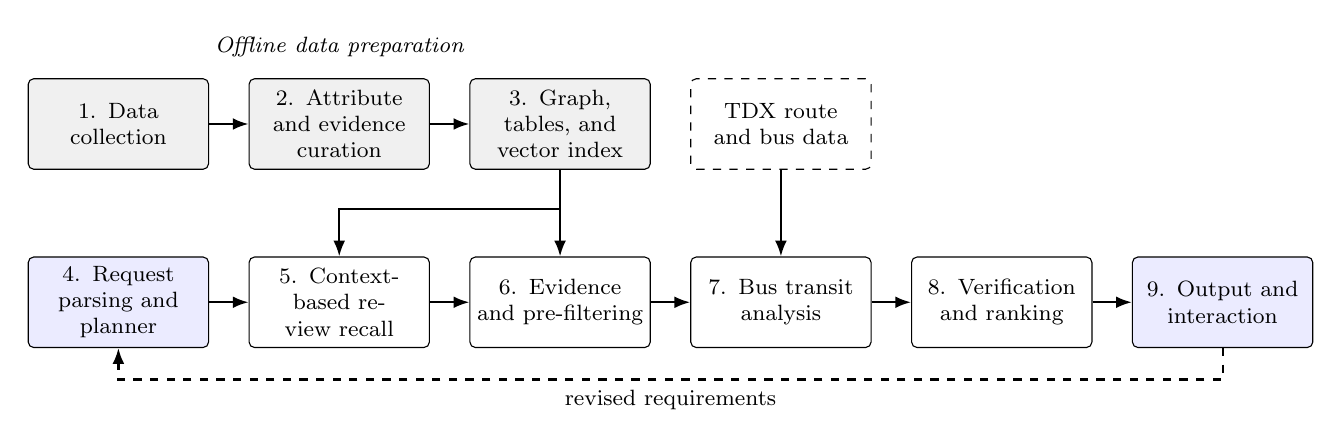
\begin{tikzpicture}[
 box/.style={draw,rounded corners=2pt,align=center,font=\footnotesize,text width=2.15cm,minimum height=1.15cm,inner sep=2pt},
 ar/.style={-{Latex[length=2mm]},thick}]
\node[box,fill=gray!12] (m1) {1. Data\\collection};
\node[box,fill=gray!12,right=0.5cm of m1] (m2) {2. Attribute and evidence curation};
\node[box,fill=gray!12,right=0.5cm of m2] (m3) {3. Graph, tables, and vector index};
\node[box,fill=blue!8,below=1.1cm of m1] (m4) {4. Request parsing and planner};
\node[box,right=0.5cm of m4] (m5) {5. Context-based review recall};
\node[box,right=0.5cm of m5] (m6) {6. Evidence and pre-filtering};
\node[box,right=0.5cm of m6] (m7) {7. Bus transit analysis};
\node[box,right=0.5cm of m7] (m8) {8. Verification and ranking};
\node[box,fill=blue!8,right=0.5cm of m8] (m9) {9. Output and interaction};
\node[box,dashed,above=1.1cm of m7] (tdx) {TDX route and bus data};
\node[font=\footnotesize\itshape,above=0.15cm of m2] {Offline data preparation};
\draw[ar] (m1)--(m2); \draw[ar] (m2)--(m3);
\draw[ar] (m3.south) -- ++(0,-0.5) -| (m5.north);
\draw[ar] (m3.south) -- ++(0,-0.5) -| (m6.north);
\draw[ar] (tdx)--(m7);
\foreach \a/\b in {m4/m5,m5/m6,m6/m7,m7/m8,m8/m9} \draw[ar] (\a)--(\b);
\draw[ar,dashed] (m9.south) -- ++(0,-0.4) -| node[pos=0.25,below,font=\footnotesize] {revised requirements} (m4.south);
\end{tikzpicture}
\caption{System architecture. Modules 1--3 prepare restaurant and evidence data offline; modules 4--9 perform online recommendation. Transit conditions are applied before the final ranking.}
\label{fig:architecture}
\end{figure*}

\subsection{Data and Evidence Management}
Table~\ref{tab:data} lists the planned data sources. Reviews are the core semantic data; their sources and permitted uses must be confirmed first. Video narration, viewer comments, and on-site reviews are labeled as different evidence types. Each record keeps its source identifier and, when available, publication, observation or update, retrieval, and validity times. Missing times remain empty. The Places API is planned only for place matching with persistent Place IDs, subject to the provider's policies~\cite{google_places_policy}.

\begin{table}[t]
\caption{Planned Data Sources}
\label{tab:data}
\centering
\footnotesize
\begin{tabularx}{\columnwidth}{@{}>{\raggedright\arraybackslash}p{0.23\columnwidth}LL@{}}
\toprule
Data & Source & Use and check \\
\midrule
Reviews & Legally obtainable reviews; YouTube text as supplement & Context matching with source passages \\
Names, branches & Public restaurant data, manual check & Avoid merging by name only \\
Hours, prices & Official information, manual check & Keep check date and price range \\
Coordinates & Traceable location data or field check & Route queries \\
Bus plans & TDX route planning & Candidate bus and walking routes \\
Arrivals, status & TDX estimated arrival (N1) & Boarding and transfer evidence \\
Stops, timetables & TDX bus data & Direction, stop order, service day \\
\bottomrule
\end{tabularx}
\end{table}

The knowledge representation distinguishes restaurants, passages, context attributes, sources, stops, and routes. Passages mention restaurants and support attributes, and each support relation carries its source and verification state. Conflicting evidence coexists rather than being overwritten. Proximity between a restaurant and a stop only suggests a transit candidate; boarding feasibility is decided by route and time analysis. A graph relation is not itself a guarantee of correctness.

\subsection{Context-Based Retrieval}
Module~5 compares keyword, vector, and hybrid retrieval. Hybrid recall fuses normalized scores:
\begin{equation}
s_{\mathrm{retrieve}}(r,q)=\lambda\, \tilde{s}_{\mathrm{BM25}}(r,q)+(1-\lambda)\,\tilde{s}_{\mathrm{vector}}(r,q),
\label{eq:hybrid}
\end{equation}
where $0\le\lambda\le1$. Passages are grouped by restaurant so that repeated passages do not let heavily reviewed restaurants dominate. The recall size $K$, minimum relevance threshold, normalization, aggregation rule, and $\lambda$ are versioned.

\subsection{Three-Valued Feasibility Verification}
Let $H(q)$ be the index set of required constraints and $E$ the available evidence. Each checker returns $h_j(r,p,q,E)\in\{T,F,U\}$, denoting pass, known violation, or insufficient evidence. The aggregate verdict is
\begin{equation}
H(r,p,q,E)=
\begin{cases}
F, & \exists j\in H(q): h_j=F,\\
T, & \forall j\in H(q): h_j=T,\\
U, & \text{otherwise}.
\end{cases}
\label{eq:verdict}
\end{equation}
Table~\ref{tab:constraints} defines the rules. Only routes in $P_T(r,q)=\{p\in P(r,o,t_{\mathrm{dep}}): H(r,p,q,E)=T\}$ enter the verified ranking. Pairs with no $F$ but at least one $U$ are listed as provisional. One failed route does not exclude a restaurant that has other routes. The verdicts are not probabilities, and a pass holds only under the adopted data and rules.

\begin{table*}[t]
\caption{Three-Valued Rules for Required Constraints}
\label{tab:constraints}
\centering
\footnotesize
\begin{tabularx}{\textwidth}{@{}>{\raggedright\arraybackslash}p{0.13\textwidth}LLL@{}}
\toprule
Constraint & Pass ($T$) & Fail ($F$) & Unknown ($U$) \\
\midrule
Meal budget & Upper bound of price range within budget & Lower bound exceeds budget & Price or unit unknown, or range straddles budget \\
Opening hours & Arrival and expected leaving fall in one valid opening interval & Arrival or dining interval known to violate hours & Missing hours, arrival, or required dining duration \\
Walking limit & All required walking satisfies the user's definition & Segment or total walking known to exceed limit & Missing segment, time, or limit definition \\
Boarding & Walk and buffer finish before the bus, within waiting limit & No permitted trip can be caught, or service does not match & Stale estimate, weak time basis, or unmatched trip \\
Transfers & Count satisfied; arrival, walk, and buffer precede next bus & Count known to exceed limit, or no connection works & Only headway known, or time unconfirmed for next leg \\
\bottomrule
\end{tabularx}
\end{table*}

If the last-order time is known, it is checked. Otherwise, the system checks only that dining ends by closing time and discloses that last order is unconfirmed. If the user explicitly requires confirmation of ordering, this becomes a required constraint and is judged $U$.

\subsection{Timeline Model}
Let $t_{\mathrm{ready}}$ be the time at which the user reaches the boarding stop with a buffer $b_{\mathrm{board}}$, and $t_{\mathrm{bus}}$ the aligned estimated or scheduled departure. Boarding requires
\begin{equation}
\begin{aligned}
t_{\mathrm{ready}}&=t_{\mathrm{dep}}+T_{\mathrm{walk\text{-}stop}}+b_{\mathrm{board}},\\
t_{\mathrm{ready}}&\le t_{\mathrm{bus}}\le t_{\mathrm{ready}}+W_{\max}.
\end{aligned}
\label{eq:boarding}
\end{equation}
For transfer $i$, with previous arrival $a_i$, transfer walk $w_i$, buffer $b_i$, and next departure $d_{i+1}$,
\begin{equation}
a_i+w_i+b_i\le d_{i+1}.
\label{eq:transfer}
\end{equation}
A normal status and an available estimate are only inputs to the verdict, and a trip that has not yet departed is not automatically $F$. Route, sub-route, direction, stop, and stop order must match, and countdown values require a known reference time. Arrival and leaving times are
\begin{equation}
\begin{aligned}
t_{\mathrm{arr}}(r,p)={}&t_{\mathrm{dep}}+T_{\mathrm{init}}+\sum_i\left(T_{\mathrm{wait},i}+T_{\mathrm{ride},i}\right)\\
&+\sum_i T_{\mathrm{transfer},i}+T_{\mathrm{final}},\\
t_{\mathrm{leave}}(r,p)={}&t_{\mathrm{arr}}(r,p)+D_{\mathrm{meal}},
\end{aligned}
\label{eq:timeline}
\end{equation}
where $T_{\mathrm{init}}$, $T_{\mathrm{transfer},i}$, and $T_{\mathrm{final}}$ are the initial, transfer, and final walking times. Segments already included in an API estimate are not added twice, and later events are recomputed when waiting or transfer times change. $D_{\mathrm{meal}}$ is preferably given by the user; a default of 90--120 minutes is a planning assumption that is displayed and editable. Overnight and split opening hours are converted into dated intervals.

\subsection{Restaurant Ranking}
Transit burden is computed separately from contextual relevance. Each verified route is scored as
\begin{equation}
\begin{aligned}
S(r,p\,|\,q)={}&\alpha s_{\mathrm{sem}}+\beta s_{\mathrm{ctx}}-\gamma c_{\mathrm{food}}-\delta u_{\mathrm{walk}}\\
&-\epsilon u_{\mathrm{wait}}-\zeta u_{\mathrm{rt}}-\eta u_{\mathrm{evid}},
\end{aligned}
\label{eq:score}
\end{equation}
where $s_{\mathrm{sem}}$ is review--request relevance, $s_{\mathrm{ctx}}$ source support for the context, $c_{\mathrm{food}}$ meal cost, $u_{\mathrm{walk}}$ and $u_{\mathrm{wait}}$ walking and waiting burdens, $u_{\mathrm{rt}}$ riding and transfer burden, and $u_{\mathrm{evid}}$ a cost reflecting the quality of evidence that is still sufficient for verification. The best route and the restaurant score are
\begin{equation}
\begin{aligned}
p^{*}(r)&=\arg\max_{p\in P_T(r,q)} S(r,p\,|\,q),\\
S_{\mathrm{rest}}(r\,|\,q)&=S(r,p^{*}(r)\,|\,q).
\end{aligned}
\label{eq:best}
\end{equation}
Cost terms may use a clipped linear scale with fixed bounds $b>a$:
\begin{equation}
N_{a,b}(x)=\min\left\{1,\max\left\{0,\frac{x-a}{b-a}\right\}\right\}.
\label{eq:norm}
\end{equation}
All terms are scaled to $[0,1]$ using development data. Weights are non-negative, sum to one, and are fixed together with bounds and thresholds before comparison. The midpoint of a price range is used only for scoring; the budget constraint is still verified on the range. Missing required evidence is never absorbed as a small penalty. Each restaurant appears once, at most three are returned, and ties are broken by a fixed identifier.

\subsection{Recommendation Algorithm}
Algorithm~\ref{alg:main} summarizes the flow. Each decision record stores the restaurant, plan, and constraint identifiers, verdict, reason, evidence identifiers, and decision time. A failed route query is recorded separately from known absence of service, and constraints are never relaxed silently.

\begin{algorithm}[t]
\caption{Context-First Recommendation with Bus Analysis}
\label{alg:main}
\footnotesize
\begin{algorithmic}[1]
\Require Request $Q$, origin $o$, departure time $t_{\mathrm{dep}}$
\Ensure Restaurants, bus plans, evidence, and unknown items
\State $q \gets$ \Call{ParseWithSchema}{$Q,o,t_{\mathrm{dep}}$}
\State \textbf{if} fields are missing or invalid \textbf{then return} a question or error
\State $C \gets$ \Call{RecallAndDeduplicate}{$q$}
\State \textbf{if} $C=\emptyset$ \textbf{then return} no contextual match
\State $E \gets$ \Call{RetrieveEvidence}{$C$}
\State $C \gets$ \Call{RemoveStaticFailures}{$C,E$}
\State $C \gets$ \Call{TopK}{$C$}
\State $V, Z, Log \gets \emptyset$
\For{each restaurant $r \in C$}
  \State $P \gets$ \Call{GetBusPlans}{$o,r,t_{\mathrm{dep}}$}
  \If{no usable plan can be established}
    \State record failure or unknown; \textbf{continue}
  \EndIf
  \For{each plan $p \in P$}
    \State $\tau \gets$ \Call{BuildTimeline}{$r,p,q$} with aligned bus data
    \State $h \gets$ \Call{CheckConstraints}{$r,p,\tau,E$}
    \State append the decision record to $Log$
    \State \textbf{if} $h=T$ \textbf{then} add scored $(r,p)$ to $V$
    \State \textbf{if} $h=U$ \textbf{then} add $(r,p)$ to $Z$
  \EndFor
\EndFor
\State $R \gets$ top three restaurants by best plan in $V$
\State \textbf{if} $R=\emptyset$ \textbf{then return} reasons, $Z$, $Log$
\State $X \gets$ \Call{Explain}{$R,Log$}
\State \textbf{if} $X$ fails fact check \textbf{then} use a template
\State \Return $R$, plans, $X$, $Z$, $Log$
\end{algorithmic}
\end{algorithm}

%=====================================================
\section{Experimental Design}\label{sec:experiments}
This section presents the planned evaluation. No experimental results are reported yet.
\subsection{Setup}
The evaluation will use Taichung restaurant data and requests covering contexts such as dates, birthday celebrations, and gatherings with friends. The compared methods will share the same restaurant facts, requests, and recorded transit data so that differences can be attributed to the method under test. Weights, thresholds, and buffers will be set on development data and fixed before testing. Contextual relevance will be judged by human annotators. The numbers of restaurants, requests, and annotators remain to be determined.

\subsection{Baselines and Metrics}
Table~\ref{tab:plan} maps each research question to its comparison and metrics. For RQ3, the violation rate is the share of verified recommendations that are found to break a required constraint, and coverage is the share of requests with at least one verified recommendation. Both are reported together, because a stricter buffer can reduce errors while sharply reducing coverage. When a method returns no recommendation at all, its violation rate is undefined rather than zero; refusals and false infeasibility are examined separately. As a further ablation, the knowledge graph will be compared with relational tables on path traceability, query correctness, latency, and maintenance cost.

\begin{table}[t]
\caption{Planned Evaluation}
\label{tab:plan}
\centering
\footnotesize
\begin{tabularx}{\columnwidth}{@{}lLL@{}}
\toprule
RQ & Comparison & Metrics \\
\midrule
1 & BM25, vector, hybrid recall & Recall@$K$, nDCG@$K$ \\
2 & Route lookup after ranking vs. transit-aware ranking & nDCG@3, walking, waiting, riding time, transfers \\
3 & Binary vs. three-valued verification with records & Violation rate, unsupported-claim rate, coverage \\
4 & Departure-time or single-estimate check vs. full timeline & Misjudged boarding, transfer, and closing cases \\
\bottomrule
\end{tabularx}
\end{table}

\subsection{Scenario Tests}
Designed cases will check the verification logic. For example, if arrival is expected at 18:50, the restaurant closes at 19:00, and dining takes 90 minutes, the expected verdict is $F$. If the last bus is due in 3 minutes but walking to the stop takes 6 minutes, the plan must not be treated as boardable. Further cases cover conflicting opening hours, unmatched arrival estimates, and requests for which no route is returned.

\subsection{Threats to Validity}
Relevance annotation is subjective, and external data may be incomplete or incorrect. Parsing errors, such as a wrong budget unit or date, can make a correct checker verify the wrong requirement; parsed fields are therefore linked to the original phrases. Replaying recorded arrival data can validate processing under changing information, but it cannot show that recommendations reduce actual missed buses; that claim would require observed arrivals and additional evidence.

%=====================================================
\section{Conclusion}\label{sec:conclusion}
This paper proposes a restaurant recommendation agent that recalls contextually matched restaurants from review evidence and applies Taichung bus conditions before the final ranking. Three-valued verification and a complete timeline separate known violations from insufficient evidence, and decision records support traceable explanations. The expected outcome is a prototype that helps users weigh contextual suitability against transit convenience; these expectations have not yet been validated. The results will depend on data coverage, parsing accuracy, and the quality of external arrival estimates. Future work includes monitoring after departure, replanning under delays, alternative restaurant suggestions, and return-trip planning.


\bibliographystyle{IEEEtran}
\bibliography{bib/ieee_paper}

\end{document}